\documentclass[zihao=-4]{ctexart}

\usepackage{amsmath}
\usepackage{graphicx}
\usepackage{float}
\usepackage{listing}
\usepackage{geometry}
\usepackage{multicol}
\usepackage{gbt7714}
\usepackage{enumerate}

\geometry{left=3cm,right=2.5cm,top=2.5cm,bottom=2.5cm}

\linespread{1.8}



\begin{document}
\begin{figure}
    \begin{minipage}{0.6\linewidth}
        
\includegraphics{pic/xiaohui.png}
    \end{minipage}
    \hfill
    \begin{minipage}{0.3\linewidth}
        组\ \ \ 别:\underline{ 本科生 }
        
        题\ \ \ 目:\underline{ B }

        队\ \ \ 号:\underline{ 030 }
    \end{minipage}
\end{figure}

\vbox{}
\vbox{}

\begin{figure}[H]
    \centering
    
\includegraphics{pic/xiaoming.png}
\end{figure}
\vbox{}
\centerline{\textbf{\Huge{2019年数学建模竞赛}}}
\vbox{}
\vbox{}
\centerline{\LARGE{biaoti}}
\vbox{}
\vbox{}
\vbox{}


\centerline{\underline{李亦龙 18373580}}\par
\centerline{\underline{叶凡 18374449}}\par
\centerline{\underline{栾帅 18373298}}\par
\centerline{队伍联系电话:\underline{13718250032}}\par
\centerline{队伍联系邮箱:\underline{18373580@buaa.edu.cn}}\par

\normalsize

\newpage
\section*{摘要}

本文基于GEO数据库公开的对于某些疾病的多个样本的基因测序结果, 


\newpage

\section*{队伍声明}

我代表参赛队伍全体队员声明,本论文及其研究工作是由队伍成员独立完成的,在完成论文时所利用的一切资料均已在参考文献中列出 
\newpage
\tableofcontents

\section{问题重述}
基因共表达网络(Gene co-expression network)是现代生物基因工程研究的重要方向, 也是研究基因与基因之间对于在某疾病上的表达影响的重要方法. 网络中节点代表基因, 节点与节点之间的连线代表基因之间的联系. 一张某疾病的基因共表达网络形如:
\begin{figure}[H]
    \centering
    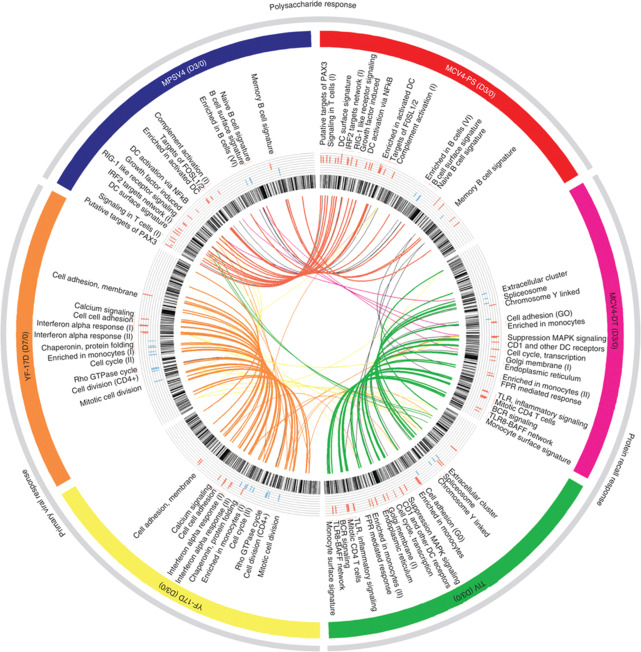
\includegraphics[width=0.6\textwidth]{pic/example.jpg}
    \caption{基因共表达网络示例\cite{example}}
\end{figure}

根据对表达出某疾病的许多样本的基因测序结果, 我们可以通过对同时出现的基因进行统计, 认为同时出现次数越多的基因可能会对该性状起阳性结果, 而出现次数较少的可以认为对该性状起阴性结果, 次数适中的认为是无关基因.
\section{假设与符号}
\subsection{假设}

\begin{enumerate}[I.]
    \item 基因与基因之间相对独立, 即全体样本中基因频率为定值
    \item 基因A与基因B之间的关系有三种: 正相关, 负相关和无关
    \item 视在实验选定的样本里出现次数多的基因对该疾病有促进作用
    \item 关于基因之间的关系, 我们认为有正相关, 负相关, 无关3种情况:
    \begin{enumerate}[i.]
        \item 认为正相关即相关系数$\rho \in [\alpha, 1]$
        \item 认为负相关为相关系数$\rho \in [-1,\alpha]$
        \item 认为无关为不属于上述二者的数据
    \end{enumerate}
\end{enumerate}

\subsection{符号}
\begin{table}[H]
    \centering
    \caption{符号说明}
    \begin{tabular}{r|l}
        \hline
        符号 & 意义\\
        \hline
        $\rho$ & 皮尔逊积矩相关系数\\
        $\alpha$ & 相关系数中的参数, 用于确定基因之间的关系\\
        \hline
    \end{tabular}
    
\end{table}



\section{问题分析}
\subsection{基因之间的联系表达}
基因之间的复杂的表达关系无法直接用数据表达, 因为基因A可能会对基因B起正相关, 对基因C起负相关, 而基因B和C对疾病都可能呈现正相关效果. 为了解释清楚这种关系, 我们将A,B,C与疾病之间的复杂关系描述为A与B, B与C, A与C之间的关系, 即相当于描述为网络中节点之间的关系.

由于基因

\subsection{等位基因}
等位基因指位于一对同源染色体相同位置上控制同一性状不同形态的基因.

在GEO数据库中, 等位基因会使用多个编号来标记, 即若A, B互为等位基因, 则A与B的ENSG编号是不同的. 这样就代表着在数据中会包含互补的数据(即等位基因). 这样的数据一般呈现A与B的出现频率相加约等于100\%的情况, 与我们认为的负相关情况类似, 所以我们不单独考虑等位基因对图中联系造成的影响.

kanbudong\cite{ranger}wosss
\section{求解问题}
\subsection{皮尔逊积矩相关系数}
对于两组数据, 我们可以利用皮尔逊积矩相关系数\cite{wiki:pierxun}来求他们之间的相似程度. 

皮尔逊积矩相关系数(Pearson product-moment correlation coefficient,又称作PPMCC或PCCs, 文章中常用r或Pearson's r表示)是一种比较非中心化数据相似程度的一种方法, 该方法的特点在于得到的结果不受线性变换的影响, 即结果与数据的单位等无关.

由于基因的测量量单位FPKM(Fragments Per Kilobase of exon model per Million mapped fragments, 每千个碱基的转录每百万映射读取的fragments)与基因本身的规模有关, 所以数据库中得到的数据的均值由于基因的变化会发生较大的升降. 为了抵消这种对数据本身的拉伸对数据特征造成的破坏, 我们选择使用皮尔逊积矩相关系数这种更加本质的特征, 它反映了两组数据在线性上的相似性, 而非数据大小. 

皮尔逊积矩相关系数的取值范围在$[-1,1]$, 假设参数$\alpha$

\begin{equation}
    \rho_{X, Y}=\frac{\operatorname{cov}(X, Y)}{\sigma_{X} \sigma_{Y}}=\frac{E\left[\left(X-\mu_{X}\right)\left(Y-\mu_{Y}\right)\right]}{\sigma_{X} \sigma_{Y}}
\end{equation}

\begin{equation}
    r=\frac{\sum_{i=1}^{n}\left(X_{i}-\overline{X}\right)\left(Y_{i}-\overline{Y}\right)}{\sqrt{\sum_{i=1}^{n}\left(X_{i}-\overline{X}\right)^{2}} \sqrt{\sum_{i=1}^{n}\left(Y_{i}-\overline{Y}\right)^{2}}}
\end{equation}

\begin{equation}
    r=\frac{1}{n-1} \sum_{i=1}^{n}\left(\frac{X_{i}-\overline{X}}{\sigma_{X}}\right)\left(\frac{Y_{i}-\overline{Y}}{\sigma_{Y}}\right)
\end{equation}

\newpage
\section*{结论}


\newpage
\section*{附录}

\bibliography{library}

\section*{支撑材料文件列表}

\end{document}
